% How the teacher's exam scope becomes a level label for one PR, and the training set.
% Generated by gen_selector_training_teacher.py; edit that script, not this file.
% Real: items, kinds, token sizes, first levels and per-level tokens of FreeCAD/FreeCAD#21257.
% Illustrative: which human comment each item supports, so the scope and the label.
% This labelling scheme is not yet written in docs/context_selector_roadmap.md.
\documentclass[tikz,border=4pt]{standalone}
\usepackage[T1]{fontenc}
\usepackage[default]{sourcesanspro}
\usepackage[scaled=0.86]{beramono}
\usepackage{amsmath,amssymb}
\usepackage{fontawesome5}
\usetikzlibrary{calc,arrows.meta,positioning,decorations.pathreplacing}

\definecolor{ink}{HTML}{1F2328}   \definecolor{grey}{HTML}{6E6A65}  \definecolor{hair}{HTML}{DEDAD4}
\definecolor{paper}{HTML}{FBFAF8}
\definecolor{inS}{HTML}{5C5751}
\definecolor{ourS}{HTML}{2E7D78}  \definecolor{ourD}{HTML}{1F5E5A}
\definecolor{llmS}{HTML}{4F5D8C}
\definecolor{accC}{HTML}{E06A4E}

\tikzset{
  >={Latex[length=2.6mm,width=2.1mm]},
  panel/.style={draw=hair!85!grey, fill=paper, line width=0.8pt, rounded corners=8pt},
  title/.style={font=\large\bfseries, anchor=base west, inner sep=0pt},
  step/.style={circle, fill=#1, text=white, font=\small\bfseries, inner sep=0pt, minimum size=0.56cm},
  sub/.style={font=\footnotesize, text=grey, anchor=north west, inner sep=0pt, align=left},
  head/.style={font=\scriptsize\bfseries, text=ink, inner sep=0pt},
  flow/.style={->, line width=1.4pt, draw=ink!75, rounded corners=6pt},
}
\newcommand{\stephead}[5]{% x, y, colour, number, title
  \node[step=#3] at (#1,#2) {#4};
  \node[title, text=#3] at ($(#1,#2)+(0.45,-0.16)$) {#5};}

\begin{document}
\begin{tikzpicture}

% ======================================================================== top row
\draw[panel] (0,0) rectangle (8.6,-7.0);
\draw[panel] (9.3,0) rectangle (14.4,-7.0);
\draw[panel] (15.1,0) rectangle (22.0,-7.0);

\stephead{0.55}{-0.6}{inS}{1}{Candidate code}
\node[sub, text width=7.8cm] at (0.3,-1.1) {FreeCAD \#21257: 10 of the pieces the tracer finds};
\stephead{9.85}{-0.6}{llmS}{2}{Teacher LLM}
\node[sub, text width=4.7cm] at (9.6,-1.1) {{\color{accC}\faKey}\; holds the solution:\\ the PR's 6 human comments, R1--R6};
\stephead{15.65}{-0.6}{accC}{3}{Exam scope}
\node[sub, text width=6.5cm] at (15.4,-1.1) {pieces some comment relies on, and the level where each piece first appears};

\node[head, anchor=west] at (1.55,-2.12) {piece of code};
\node[head, anchor=east] at (6.6,-2.12) {tokens};
\node[head] at (11.5,-2.12) {supports};
\node[head, anchor=west] at (15.6,-2.12) {in scope?};
\node[head] at (20.6,-2.12) {first level};

\fill[accC!9, rounded corners=3pt] (0.20,-2.790) rectangle (8.40,-2.410);
\fill[accC!9, rounded corners=3pt] (9.50,-2.790) rectangle (14.20,-2.410);
\fill[accC!9, rounded corners=3pt] (15.30,-2.790) rectangle (21.80,-2.410);
\node[font=\tiny\bfseries, text=grey, draw=hair!70!grey, rounded corners=1.5pt, inner sep=1.5pt, minimum width=1.0cm] at (0.9,-2.600) {changed};
\node[font=\ttfamily\fontsize{6.1}{7}\selectfont, text=accC, anchor=west, inner sep=0pt] at (1.55,-2.600) {Feature::getTopoShape};
\fill[accC, rounded corners=1pt] (6.75,-2.670) rectangle ++(0.315,0.14);
\node[font=\scriptsize, text=grey, anchor=east, inner sep=0pt] at (6.6,-2.600) {777};
\node[font=\scriptsize\bfseries, text=white, fill=llmS, rounded corners=2pt, inner sep=2pt] at (11.20,-2.600) {R1};
\node[font=\scriptsize\bfseries, text=white, fill=llmS, rounded corners=2pt, inner sep=2pt] at (11.82,-2.600) {R2};
\fill[accC] (15.75,-2.600) circle (0.12); \node[text=white, font=\tiny] at (15.75,-2.600) {\faCheck};
\node[font=\scriptsize\bfseries, text=accC, anchor=west] at (16.0,-2.600) {in scope};
\node[font=\scriptsize\bfseries, text=accC] at (20.6,-2.600) {L02};
\fill[accC!9, rounded corners=3pt] (0.20,-3.220) rectangle (8.40,-2.840);
\fill[accC!9, rounded corners=3pt] (9.50,-3.220) rectangle (14.20,-2.840);
\fill[accC!9, rounded corners=3pt] (15.30,-3.220) rectangle (21.80,-2.840);
\node[font=\tiny\bfseries, text=grey, draw=hair!70!grey, rounded corners=1.5pt, inner sep=1.5pt, minimum width=1.0cm] at (0.9,-3.030) {changed};
\node[font=\ttfamily\fontsize{6.1}{7}\selectfont, text=accC, anchor=west, inner sep=0pt] at (1.55,-3.030) {Hole::execute};
\fill[accC, rounded corners=1pt] (6.75,-3.100) rectangle ++(0.061,0.14);
\node[font=\scriptsize, text=grey, anchor=east, inner sep=0pt] at (6.6,-3.030) {150};
\node[font=\scriptsize\bfseries, text=white, fill=llmS, rounded corners=2pt, inner sep=2pt] at (11.20,-3.030) {R3};
\fill[accC] (15.75,-3.030) circle (0.12); \node[text=white, font=\tiny] at (15.75,-3.030) {\faCheck};
\node[font=\scriptsize\bfseries, text=accC, anchor=west] at (16.0,-3.030) {in scope};
\node[font=\scriptsize\bfseries, text=accC] at (20.6,-3.030) {L02};
\node[font=\tiny\bfseries, text=grey, draw=hair!70!grey, rounded corners=1.5pt, inner sep=1.5pt, minimum width=1.0cm] at (0.9,-3.460) {changed};
\node[font=\ttfamily\fontsize{6.1}{7}\selectfont, text=ink, anchor=west, inner sep=0pt] at (1.55,-3.460) {ProfileBased::getProfileShape};
\fill[hair, rounded corners=1pt] (6.75,-3.530) rectangle ++(0.094,0.14);
\node[font=\scriptsize, text=grey, anchor=east, inner sep=0pt] at (6.6,-3.460) {232};
\node[font=\scriptsize, text=hair!60!grey] at (11.2,-3.460) {--};
\draw[hair!80!grey, line width=0.8pt] (15.75,-3.460) circle (0.11);
\node[font=\scriptsize, text=grey, anchor=west] at (16.0,-3.460) {not needed};
\node[font=\scriptsize, text=grey] at (20.6,-3.460) {L02};
\fill[accC!9, rounded corners=3pt] (0.20,-4.080) rectangle (8.40,-3.700);
\fill[accC!9, rounded corners=3pt] (9.50,-4.080) rectangle (14.20,-3.700);
\fill[accC!9, rounded corners=3pt] (15.30,-4.080) rectangle (21.80,-3.700);
\node[font=\tiny\bfseries, text=grey, draw=hair!70!grey, rounded corners=1.5pt, inner sep=1.5pt, minimum width=1.0cm] at (0.9,-3.890) {callee};
\node[font=\ttfamily\fontsize{6.1}{7}\selectfont, text=accC, anchor=west, inner sep=0pt] at (1.55,-3.890) {Hole::findHoles};
\fill[accC, rounded corners=1pt] (6.75,-3.960) rectangle ++(0.271,0.14);
\node[font=\scriptsize, text=grey, anchor=east, inner sep=0pt] at (6.6,-3.890) {668};
\node[font=\scriptsize\bfseries, text=white, fill=llmS, rounded corners=2pt, inner sep=2pt] at (11.20,-3.890) {R3};
\fill[accC] (15.75,-3.890) circle (0.12); \node[text=white, font=\tiny] at (15.75,-3.890) {\faCheck};
\node[font=\scriptsize\bfseries, text=accC, anchor=west] at (16.0,-3.890) {in scope};
\node[font=\scriptsize\bfseries, text=accC] at (20.6,-3.890) {L04};
\node[font=\tiny\bfseries, text=grey, draw=hair!70!grey, rounded corners=1.5pt, inner sep=1.5pt, minimum width=1.0cm] at (0.9,-4.320) {callee};
\node[font=\ttfamily\fontsize{6.1}{7}\selectfont, text=ink, anchor=west, inner sep=0pt] at (1.55,-4.320) {Hole::makeThread};
\fill[hair, rounded corners=1pt] (6.75,-4.390) rectangle ++(0.633,0.14);
\node[font=\scriptsize, text=grey, anchor=east, inner sep=0pt] at (6.6,-4.320) {1,561};
\node[font=\scriptsize, text=hair!60!grey] at (11.2,-4.320) {--};
\draw[hair!80!grey, line width=0.8pt] (15.75,-4.320) circle (0.11);
\node[font=\scriptsize, text=grey, anchor=west] at (16.0,-4.320) {not needed};
\node[font=\scriptsize, text=grey] at (20.6,-4.320) {L04};
\node[font=\tiny\bfseries, text=grey, draw=hair!70!grey, rounded corners=1.5pt, inner sep=1.5pt, minimum width=1.0cm] at (0.9,-4.750) {callee};
\node[font=\ttfamily\fontsize{6.1}{7}\selectfont, text=ink, anchor=west, inner sep=0pt] at (1.55,-4.750) {Measurement::getShape};
\fill[hair, rounded corners=1pt] (6.75,-4.820) rectangle ++(0.040,0.14);
\node[font=\scriptsize, text=grey, anchor=east, inner sep=0pt] at (6.6,-4.750) {99};
\node[font=\scriptsize, text=hair!60!grey] at (11.2,-4.750) {--};
\draw[hair!80!grey, line width=0.8pt] (15.75,-4.750) circle (0.11);
\node[font=\scriptsize, text=grey, anchor=west] at (16.0,-4.750) {not needed};
\node[font=\scriptsize, text=grey] at (20.6,-4.750) {L04};
\fill[accC!9, rounded corners=3pt] (0.20,-5.370) rectangle (8.40,-4.990);
\fill[accC!9, rounded corners=3pt] (9.50,-5.370) rectangle (14.20,-4.990);
\fill[accC!9, rounded corners=3pt] (15.30,-5.370) rectangle (21.80,-4.990);
\node[font=\tiny\bfseries, text=grey, draw=hair!70!grey, rounded corners=1.5pt, inner sep=1.5pt, minimum width=1.0cm] at (0.9,-5.180) {caller};
\node[font=\ttfamily\fontsize{6.1}{7}\selectfont, text=accC, anchor=west, inner sep=0pt] at (1.55,-5.180) {ProfileBased::getTopoShapeProfileWires};
\fill[accC, rounded corners=1pt] (6.75,-5.250) rectangle ++(0.105,0.14);
\node[font=\scriptsize, text=grey, anchor=east, inner sep=0pt] at (6.6,-5.180) {260};
\node[font=\scriptsize\bfseries, text=white, fill=llmS, rounded corners=2pt, inner sep=2pt] at (11.20,-5.180) {R4};
\fill[accC] (15.75,-5.180) circle (0.12); \node[text=white, font=\tiny] at (15.75,-5.180) {\faCheck};
\node[font=\scriptsize\bfseries, text=accC, anchor=west] at (16.0,-5.180) {in scope};
\node[font=\scriptsize\bfseries, text=accC] at (20.6,-5.180) {L05};
\node[font=\tiny\bfseries, text=grey, draw=hair!70!grey, rounded corners=1.5pt, inner sep=1.5pt, minimum width=1.0cm] at (0.9,-5.610) {caller};
\node[font=\ttfamily\fontsize{6.1}{7}\selectfont, text=ink, anchor=west, inner sep=0pt] at (1.55,-5.610) {CmdPartReverseShape::isActive};
\fill[hair, rounded corners=1pt] (6.75,-5.680) rectangle ++(0.035,0.14);
\node[font=\scriptsize, text=grey, anchor=east, inner sep=0pt] at (6.6,-5.610) {86};
\node[font=\scriptsize, text=hair!60!grey] at (11.2,-5.610) {--};
\draw[hair!80!grey, line width=0.8pt] (15.75,-5.610) circle (0.11);
\node[font=\scriptsize, text=grey, anchor=west] at (16.0,-5.610) {not needed};
\node[font=\scriptsize, text=grey] at (20.6,-5.610) {L05};
\node[font=\tiny\bfseries, text=grey, draw=hair!70!grey, rounded corners=1.5pt, inner sep=1.5pt, minimum width=1.0cm] at (0.9,-6.040) {guide};
\node[font=\ttfamily\fontsize{6.1}{7}\selectfont, text=ink, anchor=west, inner sep=0pt] at (1.55,-6.040) {CONTRIBUTING.md};
\fill[hair, rounded corners=1pt] (6.75,-6.110) rectangle ++(0.900,0.14);
\node[font=\scriptsize, text=grey, anchor=east, inner sep=0pt] at (6.6,-6.040) {2,221};
\node[font=\scriptsize, text=hair!60!grey] at (11.2,-6.040) {--};
\draw[hair!80!grey, line width=0.8pt] (15.75,-6.040) circle (0.11);
\node[font=\scriptsize, text=grey, anchor=west] at (16.0,-6.040) {not needed};
\node[font=\scriptsize, text=grey] at (20.6,-6.040) {L07};
\node[font=\tiny\bfseries, text=grey, draw=hair!70!grey, rounded corners=1.5pt, inner sep=1.5pt, minimum width=1.0cm] at (0.9,-6.470) {test};
\node[font=\ttfamily\fontsize{6.1}{7}\selectfont, text=ink, anchor=west, inner sep=0pt] at (1.55,-6.470) {TopoShapeMakeShape...Tests};
\fill[hair, rounded corners=1pt] (6.75,-6.540) rectangle ++(0.115,0.14);
\node[font=\scriptsize, text=grey, anchor=east, inner sep=0pt] at (6.6,-6.470) {285};
\node[font=\scriptsize, text=hair!60!grey] at (11.2,-6.470) {--};
\draw[hair!80!grey, line width=0.8pt] (15.75,-6.470) circle (0.11);
\node[font=\scriptsize, text=grey, anchor=west] at (16.0,-6.470) {not needed};
\node[font=\scriptsize, text=grey] at (20.6,-6.470) {L09};

\draw[flow] (8.62,-0.6) -- (9.28,-0.6);
\draw[flow] (14.42,-0.6) -- (15.08,-0.6);

% ======================================================================== bottom row
\draw[panel] (0,-7.7) rectangle (12.4,-11.5);
\draw[panel] (13.1,-7.7) rectangle (22.0,-11.5);

\stephead{0.55}{-8.3}{accC}{4}{From exam scope to a level}
\node[sub, text width=11.6cm] at (0.3,-8.8) {the label is the smallest nested level that contains every in-scope piece};
\draw[draw=accC!40, fill=accC!14, line width=0.7pt, rounded corners=3pt] (0.750,-10.35) rectangle ++(0.980,0.8);
\node[font=\scriptsize\bfseries, text=ink] at (1.240,-9.75) {L01};
\node[font=\tiny, text=grey] at (1.240,-10.12) {13k};
\draw[draw=accC!40, fill=accC!14, line width=0.7pt, rounded corners=3pt] (1.880,-10.35) rectangle ++(0.980,0.8);
\node[font=\scriptsize\bfseries, text=ink] at (2.370,-9.75) {L02};
\node[font=\tiny, text=grey] at (2.370,-10.12) {41k};
\fill[accC] (2.250,-9.3) circle (0.085);
\fill[accC] (2.490,-9.3) circle (0.085);
\draw[draw=accC!40, fill=accC!14, line width=0.7pt, rounded corners=3pt] (3.010,-10.35) rectangle ++(0.980,0.8);
\node[font=\scriptsize\bfseries, text=ink] at (3.500,-9.75) {L03};
\node[font=\tiny, text=grey] at (3.500,-10.12) {64k};
\draw[draw=accC!40, fill=accC!14, line width=0.7pt, rounded corners=3pt] (4.140,-10.35) rectangle ++(0.980,0.8);
\node[font=\scriptsize\bfseries, text=ink] at (4.630,-9.75) {L04};
\node[font=\tiny, text=grey] at (4.630,-10.12) {78k};
\fill[accC] (4.630,-9.3) circle (0.085);
\draw[draw=accC, fill=accC!14, line width=1.4pt, rounded corners=3pt] (5.270,-10.35) rectangle ++(0.980,0.8);
\node[font=\scriptsize\bfseries, text=accC] at (5.760,-9.75) {L05};
\node[font=\tiny, text=grey] at (5.760,-10.12) {87k};
\fill[accC] (5.760,-9.3) circle (0.085);
\draw[draw=hair!80!grey, fill=white, line width=0.7pt, rounded corners=3pt] (6.400,-10.35) rectangle ++(0.980,0.8);
\node[font=\scriptsize\bfseries, text=ink] at (6.890,-9.75) {L06};
\node[font=\tiny, text=grey] at (6.890,-10.12) {87k};
\draw[draw=hair!80!grey, fill=white, line width=0.7pt, rounded corners=3pt] (7.530,-10.35) rectangle ++(0.980,0.8);
\node[font=\scriptsize\bfseries, text=ink] at (8.020,-9.75) {L07};
\node[font=\tiny, text=grey] at (8.020,-10.12) {91k};
\draw[draw=hair!80!grey, fill=white, line width=0.7pt, rounded corners=3pt] (8.660,-10.35) rectangle ++(0.980,0.8);
\node[font=\scriptsize\bfseries, text=ink] at (9.150,-9.75) {L08};
\node[font=\tiny, text=grey] at (9.150,-10.12) {118k};
\draw[draw=hair!80!grey, fill=white, line width=0.7pt, rounded corners=3pt] (9.790,-10.35) rectangle ++(0.980,0.8);
\node[font=\scriptsize\bfseries, text=ink] at (10.280,-9.75) {L09};
\node[font=\tiny, text=grey] at (10.280,-10.12) {119k};
\draw[draw=hair!80!grey, fill=white, line width=0.7pt, rounded corners=3pt] (10.920,-10.35) rectangle ++(0.980,0.8);
\node[font=\scriptsize\bfseries, text=ink] at (11.410,-9.75) {L10};
\node[font=\tiny, text=grey] at (11.410,-10.12) {256k};
\draw[decorate, decoration={brace, amplitude=5pt, mirror}, line width=1pt, draw=accC] (0.750,-10.47) -- (6.250,-10.47);
\node[font=\small, anchor=north west, inner sep=0pt] at (0.750,-10.75) {\textbf{\color{accC}label = L05}\quad{\color{grey}\footnotesize 87k tokens, instead of 256k for L10}};
\node[font=\scriptsize, text=accC, anchor=west] at (6.400,-9.3) {$\bullet$ an in-scope item, at the level it first appears};

\stephead{13.65}{-8.3}{ourS}{5}{Training set}
\node[sub, text width=8.2cm] at (13.4,-8.8) {input: the PR, never the solution \;$\cdot$\; target: its level};
\draw[hair!85!grey, line width=0.6pt] (13.45,-9.55) -- (19.5,-9.55);
\node[head, anchor=west] at (13.5,-9.33) {training PR (input $\mathbf{x}$)};
\node[head] at (18.95,-9.33) {level $y$};
\fill[accC!9, rounded corners=3pt] (13.4,-9.93) rectangle (19.5,-9.57);
\node[font=\scriptsize, text=ink, anchor=west] at (13.5,-9.75) {FreeCAD \#21257 \;{\color{grey}Fix hole centered on point}};
\node[font=\scriptsize\bfseries, text=white, fill=accC, rounded corners=1.5pt, inner sep=2pt] at (18.95,-9.75) {L05};
\node[font=\scriptsize, text=ink, anchor=west] at (13.5,-10.2) {FreeCAD \#19411 \;{\color{grey}TechDraw: hard type enums}};
\node[font=\scriptsize, text=grey] at (18.95,-10.2) {$\cdots$};
\node[font=\scriptsize, text=grey, anchor=west] at (13.5,-10.65) {$\ldots$ 196 PRs from 50 repositories};

\node[circle, fill=ourD, text=white, minimum size=1.35cm, align=center, font=\small\bfseries] (sel) at (20.85,-9.85) {Selector\\[-3pt]$f_\theta$};
\node[font=\scriptsize, text=grey, anchor=north] at (20.85,-10.6) {learns PR $\mapsto$ level};
\draw[flow, draw=ourD] (19.55,-9.85) -- (sel.west);

% flow between rows
\draw[flow] (18.55,-7.02) -- (18.55,-7.35) -- (6.2,-7.35) -- (6.2,-7.68);
\draw[flow] (12.42,-9.6) -- (13.08,-9.6);

\node[font=\scriptsize\itshape, text=grey, anchor=north east, inner sep=0pt] at (22.0,-11.65) {pieces, tokens and levels are real; the teacher's links, and so the label, are illustrative};

\end{tikzpicture}
\end{document}
